% !TEX encoding = UTF-8

%% Davide Imola - VR386238
%% Esame di LaTeX

\documentclass[a4paper,titlepage]{book}

\usepackage[english,italian]{babel}
\usepackage[nowrite,noadvisor]{frontespizio}
\usepackage{amsmath,amssymb,graphicx}
\usepackage{natbib}
\usepackage{url}
\usepackage{lipsum}
\usepackage{hyphenat}
\usepackage{url}
\usepackage{listings}

\newcommand\abstractname{Abstract}  %%% here
\makeatletter
\if@titlepage
  \newenvironment{abstract}{%
      \titlepage
      \null\vfil
      \@beginparpenalty\@lowpenalty
      \begin{center}%
        \bfseries \abstractname
        \@endparpenalty\@M
      \end{center}}%
     {\par\vfil\null\endtitlepage}
\else
  \newenvironment{abstract}{%
      \if@twocolumn
        \section*{\abstractname}%
      \else
        \small
        \begin{center}%
          {\bfseries \abstractname\vspace{-.5em}\vspace{\z@}}%
        \end{center}%
        \quotation
      \fi}
      {\if@twocolumn\else\endquotation\fi}
\fi
\makeatother


\hyphenation{Ionic}
\hyphenation{Apache CouchDB}


\begin{document}

\pagestyle{plain}

%Generazione Frontespizio
\begin{frontespizio}
\Universita{Verona}
\Dipartimento{Informatica}
\Corso[Laurea]{Informatica}
\Annoaccademico{2016--2017}
\Titoletto{Tesi di Laurea Triennale}
\Titolo{Applicazione di Coaching in Ionic con interazione a DataBase NoSQL}
\Candidato[VR386238]{Davide Imola}
\Relatore{Prof. Graziano Pravadelli}
\Correlatore{Dott. Florenc Demrozi}
\end{frontespizio}

% Front
\frontmatter

% Generazione Sommario
\begin{abstract}
La presente tesi \`{e} una documentazione del codice relativo al progetto dell'applicazione per {\foreignlanguage{english} Smartphone} di {\foreignlanguage{english} coaching}. 

In questo documento si vedr\`{a} nel dettaglio la parte relativa all'applicativo scritto in Ionic 3 e l'interazione al {\foreignlanguage{english} DataBase NoSQL} Apache CouchDB.

Nei primi capitoli si vedranno quali componenti sono stati utilizzati per la strutturazione del progetto e delle semplici guide relative alla loro installazione e corretta configurazione.

Nei capitoli restanti andremmo a coprire invece diversi aspetti di studio e progettazione del codice, partendo dall'ideazione di una base per l'interfaccia grafica alla vera e propria stesura del codice.
\end{abstract}

% Generazione Indice
\tableofcontents

%Main
\mainmatter
% Capitolo 1
\chapter{Ambiente di sviluppo}


\section{Node.js}
Per prima cosa andiamo a osservare l'installazione di Node.js, piattaforma {\foreignlanguage{english} event-driven} per il motore JavaScript V8 di Chrome. Bisogna quindi andare a scaricare dal sito \url{https://nodejs.org/en/} la versione corrente.

Al termine dell'installazione sar\`{a} presente sul vostro sistema il {\foreignlanguage{english} node package manager} richiamabile da terminale con il comando
\begin{lstlisting}[language=bash]
  $ npm
\end{lstlisting}
che utilizzeremo successivamente.

\section{Ionic 3}
Per lo sviluppo della nostra applicazione si \`{e} utilizzato principalmente Ionic nella sua versione 3, un famoso e completo {\foreignlanguage{english} SDK open-source} per lo sviluppo di applicazioni ibride per dispositivi mobili. 
Ionic 3 si basa sull'uso di AngularJS e Apache Cordova e utilizza alcune tecnologie inerenti allo sviluppo {\foreignlanguage{english} Web} come CSS, HTML5 e Sass.

Per eseguire l'installazione basta semplicemente lanciare nel proprio terminale il seguente comando
\begin{lstlisting}[language=bash]
  $ npm install -g cordova ionic
\end{lstlisting}

Questo framework permette quindi di costruire il core di un'applicazione in modo indipendente dall'architettura sottostante. Ionic permette inoltre l'inserimento di funzioni scritte in codice nativo, che sia esso Java nel caso di Android o Swift per iOS. Relativamente a queste informazioni si lasciano i seguenti articoli di approfondimento:

\url{http://devgirl.org/2013/09/17/how-to-write-a-phonegap-3-0-plugin-for-android/}

\url{http://sciencevikinglabs.com/writing-android-ionic-plugins/}

\url{https://moduscreate.com/blog/writing-a-cordova-plugin-in-swift-3-for-ios/}

\section{Apache CouchDB}
Apache CouchDB, chiamato pi\`{u} semplicemente CouchDB, \`{e} un sistema gestionale di basi di dati non relazionale. Questo \`{e} uno tra i principali sistemi NoSQL a documenti, dove questi vengono memorizzati nel formato JSON.

\section{PostgreSQL}
PostgreSQL \`{e} un completo DBMS ad oggetti rilasciato con licenza libera (stile Licenza BSD). Spesso viene abbreviato come "Postgres", sebbene questo sia un nome vecchio dello stesso progetto.

PostgreSQL \`{e} una reale alternativa sia rispetto ad altri prodotti liberi come MySQL, Firebird SQL e MaxDB che a quelli a codice chiuso come Oracle, IBM Informix o DB2 ed offre caratteristiche uniche nel suo genere che lo pongono per alcuni aspetti all'avanguardia nel settore dei database. 


\section{Python 3}
Python \`{e} un linguaggio di programmazione ad alto livello, orientato agli oggetti, adatto, tra gli altri usi, per sviluppare applicazioni distribuite, scripting, computazione numerica e system testing. 

All'interno di tutte le repository Python, oltre allo script \`{e} presente un file \textit{requirements.txt} contenente i pacchetti necessari per il corretto funzionamento.

\section{Git e GitLab}
Git \`{e} un sistema di controllo versione distribuito disponibile sia da linea di comando, che da interfaccia grafica (tra i tanti disponibili consiglio SmartGit \url{https://www.syntevo.com/smartgit/}).

Mentre GitLab \`{e} un gestore web di repository Git, dove sono stati opportunamente inseriti i codici sorgente dell'applicazione sviluppata.

% Capitolo 2
\chapter{Basi di Dati}

\section{Autenticazione basata su PostgreSQL}
Per l'autenticazione all'applicazione \`{e} stato utilizzato a tale scopo una semplice base di dati relazionale denominata \textit{coachapp} in PostgreSQL, contenente l'unica tabella \textit{users} della quale lascio la struttura in formato SQL:
\begin{lstlisting}[language=SQL,
           showspaces=false,
           basicstyle=\ttfamily,
           numbers=left,
           numberstyle=\tiny,
           commentstyle=\color{gray}]
CREATE DOMAIN groups AS VARCHAR 
	CHECK(VALUE IN('coachee','caregiver'));
	
CREATE TABLE users (
	fiscalcode VARCHAR PRIMARY KEY,
	password VARCHAR NOT NULL,
	usertype groups NOT NULL
);
\end{lstlisting}

Per l'interfacciamento a questa base di dati \`{e} stata sviluppata una API RESTful in Python, andando ad utilizzare principalmente \textit{Flask} per l'applicativo Web e \textit{psycopg2} per l'esecuzione delle Query. I routing attualmente disponibili sono \url{http://localhost/api/login} e \url{http://localhost/api/register} con i relativi parametri passabili sia in POST che in GET, ovvero \textit{user} e \textit{psw} nel caso del login e si aggiunge solamente \textit{type} nel caso register.

Tutte le password all'interno del database vengono, per ragioni di sicurezza, memorizzate sotto forma di hash SHA256 eseguito direttamente lato client in Ionic.

\section{Apache CouchDB e PouchDB}
Per la gestione delle informazioni ci siamo affidati a CouchDB, sistema NoSQL a documenti JSON. L'infrastruttura \`{e} composta da due database uno destinato ai \textit{caregivers} e uno per i \textit{coachees}. Questi rimangono costantemente sincronizzati grazie a uno script Python.

La struttura base del documento JSON per il database \textit{caregivers} \`{e} la \ref{lis:caregivers}, mentre per i \textit{coachees} la \ref{lis:coachees}.

\pagebreak
\begin{lstlisting}[showspaces=false,
           basicstyle=\ttfamily,
           numbers=left,
           numberstyle=\tiny,
           commentstyle=\color{gray},
	  captionpos=b,
	  caption=Struttura documento caregivers,
	  label=lis:caregivers]
{
  "_id": "RSSMRA90T25L781O", 
  "name": "Mario", 
  "surname": "Rossi",
  "birth": "1990-12-25",
  "coachees": {
    "BNCLNZ50B02L781Y": {
      "name": "Lorenzo",
      "surname" : "Bianchi", 
      "birth": "1950-02-02",
      "insert": "2018-02-03", 
      "pathologies": {
        "general": {
          "date_of_diagnosis" : "2018-02-03",
          "Coach Action": {
            "counter": "2",
            "coachevent1": { 
              "start_time": "12:41:56", 
              "end_time": "12:41:56"
            },
            "coachevent2": {
              "start_time": "12:41:56",
              "end_time": "12:41:56"
            },
            "done": { 
              "2018-02-03": "2 3 10"
            }
          }
        }
      }
    }
  }
}
\end{lstlisting}

\pagebreak
\begin{lstlisting}[showspaces=false,
           basicstyle=\ttfamily,
           numbers=left,
           numberstyle=\tiny,
           commentstyle=\color{gray},
	  captionpos=b,
	  caption=Struttura documento coachees,
	  label=lis:coachees]
{
  "_id": "RSSMRA90T25L781O", 
  "name": "Mario", /
  "surname": "Rossi", 
  "birth": "1990-12-25",
   "pathologies": {
        "general": { 
          "date_of_diagnosis" : "2018-02-03", 
          "Bere Acqua": { 
            "counter": "2", 
            "coachevent1": { 
              "start_time": "12:41:56", 
              "end_time": "12:41:56"
            },
            "coachevent2": {
              "start_time": "12:41:56",
              "end_time": "12:41:56"
            },
            "done": { 
              "2018-02-03": "2 3 10"
            }
          }
        }
      }
    }
  }
}
\end{lstlisting}

Inoltre su Ionic \`{e} presente un Database locale in PouchDB, il quale viene utilizzato, per effettuare le modifiche prima in locale per poi sincronizzarle con la base di dati remota. Onde evitare un database locale troppo amplio si \`{e} deciso di effettuare una sincronizzazione filtrata dei vari documenti anche per non permettere l'accesso a documenti propri per questioni di privacy. 

Per effettuarla bisogna andare a inserire nel database il design document \ref{lis:ddoc}, il quale viene richiamato dalla funzione di sincronizzazione in Ionic \ref{lis:ionicsync}.
\begin{lstlisting}[showspaces=false,
           basicstyle=\ttfamily,
           numbers=left,
           numberstyle=\tiny,
           commentstyle=\color{gray},
	  captionpos=b,
	  caption=Design document,
	  label=lis:ddoc]
{
  "_id": "_design/fiscal",
  "filters": {
    "by_id": "function(doc, req) { 
			return doc._id === req.query._id; 
		}"
  }
}

\end{lstlisting}

\pagebreak
\begin{lstlisting}[language=Java,
	  captionpos=b,
	  caption=Funzione di sincronizzazione,
	  label=lis:ionicsync]
this._LOCAL_CAREGIVERS.sync(this._REMOTE_CAREGIVERS, {
      live: true,
      retry: true,
      filter: 'fiscal/by_id',
      query_params: { "_id": this._LOGGED_USER },
      heartbeat: '1000'
    }).on('complete', function (err) {
      console.log('BD Sync Complete');
    }).on('change', function (change) {
      // yo, something changed!
      console.log('DB Sync Change');
    }).on('paused', function (info) {
      // replication was paused, 
     // usually because of a lost connection
    }).on('active', function (info) {
      // replication was resumed
    }).on('error', function (err) {
      // totally unhandled error (shouldn't happen)
    });
\end{lstlisting}

\chapter{Codice sorgente}
\section{Uso della repository}
All'interno del gruppo di GitLab si possono trovare tutte le repository dei codici sorgenti. Come primo sviluppo si sono decisi di usare due branch, il \textit{master} o \textit{stable} contenente la versione correttamente rilasciata e funzionante del software e il branch \textit{develop} contenente la parte dei sorgenti attualmente in corso di sviluppo.

Questo sistema di gestione di branch \`{e} stato utilizzato per poi lasciare la possibilità di passare a un sistema di gestione branch con pull request pi\`{u} efficiente, come ad esempio \textit{Git flow} e il suo schema (\figurename~\ref{fig:git_flow}).

\begin{figure}
\center
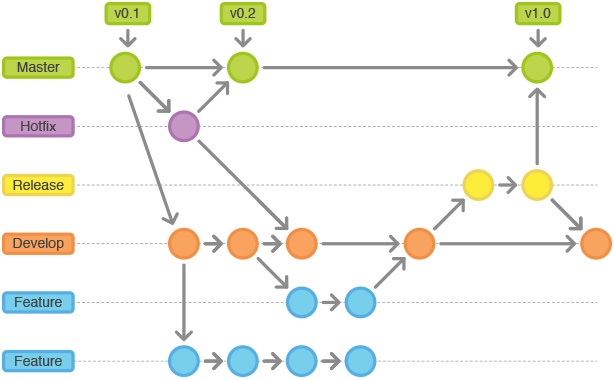
\includegraphics[width=250px]{imgs/git_flow.png}
\caption{Schema git flow \label{fig:git_flow}}
\end{figure} 

\end{document}